\section{Kết quả}\label{sec:results}

\subsection{Các benchmark}
Trong {{n_pairs}} sự kiện sửa, {{real_ok}} qua được kiểm tra hai đầu mút và {{real_one_minimal}} đạt bản sửa 1-tối thiểu trong ngân sách thử; {{real_small_repair_pct}}\% bản sửa tối thiểu chỉ thay đổi một hoặc hai hunk (\cref{fig:flow}A). {{multi_share}}\% bản sửa tối thiểu trải trên nhiều loại và bị loại khỏi tập nhãn chuẩn; {{n_real_gold}} item đơn cơ chế còn lại chủ yếu thuộc loại văn bản in (khóa học chấm output khớp từng byte), tiếp theo là biểu thức tính, thiếu bước, điều kiện rẽ nhánh, biên vòng lặp, định dạng in và luồng điều khiển ({{audit_control_flow_return}} trong {{audit_control_flow}} bản sửa luồng điều khiển được audit là thêm \texttt{return 0} mà C90 cần để có mã thoát 0). Benchmark kiểm soát gồm {{n_injected}} mutant thuộc chín loại; {{injected_equivalent_pct}}\% mutant ứng viên vẫn đạt mọi test và bị loại vì tương đương trên bộ test (\cref{fig:flow}B). \Cref{tab:hyp} tóm tắt các giả thuyết đã đăng ký; các mục tiếp theo lần lượt trả lời từng câu hỏi nghiên cứu.

\begin{table}[t]
\centering
\caption{Các giả thuyết đã đăng ký: chênh lệch trung bình trên các cohort, khoảng bootstrap 95\% và kết luận (H1a báo cáo chính trần trung bình theo kết quả test). H2 và H3 được báo cáo cho K-means và HAC.}\label{tab:hyp}
\small
\resizebox{\textwidth}{!}{%
\begin{tabular}{lrllrll}
\toprule
 & \multicolumn{3}{c}{Bản sửa thật} & \multicolumn{3}{c}{Mutant tiêm lỗi} \\
\cmidrule(lr){2-4}\cmidrule(lr){5-7}
Giả thuyết & TB & KTC 95\% & Kết luận & TB & KTC 95\% & Kết luận \\
\midrule
{{table_hypotheses}}
\bottomrule
\end{tabular}}
\end{table}

\subsection{RQ1: chữ ký test trộn lẫn cơ chế}
Các chữ ký test giống hệt thường che giấu những cơ chế khác nhau (\cref{fig:ceiling}). Tốt nhất, một hàm bất kỳ của OAV kết quả test chỉ gán đúng cơ chế cho {{real_H1a_pct}}\% bài thật (trần trung bình {{real_H1a_mean}}, KTC 95\% [{{real_H1a_lo}}; {{real_H1a_hi}}]) và {{injected_H1a_pct}}\% bài tiêm lỗi ([{{injected_H1a_lo}}; {{injected_H1a_hi}}]), nên H1a được ủng hộ trên cả hai benchmark. Nói cách khác, {{real_collision_pct}}\% trong {{real_same_signature_pairs}} cặp bài thật có cùng chữ ký test trong một bài tập là khác cơ chế, và tỷ lệ này là {{injected_collision_pct}}\% trong {{injected_same_signature_pairs}} cặp tiêm lỗi. Phần mịn thêm của OAV độ lệch nâng trần thêm {{real_H1b_mean}} [{{real_H1b_lo}}; {{real_H1b_hi}}] trên bài thật và {{injected_H1b_mean}} [{{injected_H1b_lo}}; {{injected_H1b_hi}}] trên bài tiêm lỗi so với một phân hoạch ngẫu nhiên cùng độ mịn (H1b được ủng hộ; $p$ hiệu chỉnh Holm $p {{real_H1b_p}}$ và $p {{injected_H1b_p}}$). Vậy các phân biệt thêm vào mang thông tin cơ chế chứ không chỉ tăng độ phân giải.

\begin{figure}[tbp]
\centering
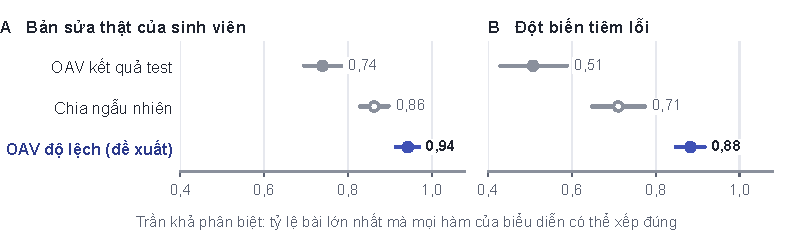
\includegraphics[width=\textwidth]{figures/fig4_ceiling_vi.pdf}
\caption{RQ1. Trần khả phân biệt của OAV kết quả test, của một phân hoạch ngẫu nhiên chia mỗi nhóm kết quả test thành các nhóm con có cùng kích thước như OAV độ lệch (vòng tròn rỗng), và của OAV độ lệch. Điểm là trung bình trên các cohort; thanh là khoảng bootstrap 95\%.}\label{fig:ceiling}
\end{figure}

\subsection{RQ2: phân cụm theo cơ chế}
\Cref{tab:ari,fig:ari} báo cáo mức khôi phục cơ chế ở cùng ngân sách phân cụm. Trên benchmark kiểm soát, cụm của OAV kết quả test hầu như không khớp với cơ chế (ARI {{injected_ari_outcomes}}, chữ ký trùng khớp {{injected_ari_exact}}), trong khi OAV độ lệch đạt {{injected_ari_deviation}}: chênh lệch {{injected_H2_kmeans_mean}} [{{injected_H2_kmeans_lo}}; {{injected_H2_kmeans_hi}}] với K-means và {{injected_H2_hac_mean}} [{{injected_H2_hac_lo}}; {{injected_H2_hac_hi}}] với HAC, cao hơn ở {{injected_H2_kmeans_wins}} cohort. Trên bản sửa thật, OAV kết quả test đã đạt {{real_ari_outcomes}} vì loại văn bản in chiếm đa số tạo ra chữ ký đặc trưng; OAV độ lệch đạt {{real_ari_deviation}} với K-means và {{real_arihac_deviation}} với HAC, nhưng các chênh lệch ({{real_H2_kmeans_mean}}, KTC [{{real_H2_kmeans_lo}}; {{real_H2_kmeans_hi}}]; {{real_H2_hac_mean}}, KTC [{{real_H2_hac_lo}}; {{real_H2_hac_hi}}]) không đáng tin cậy. Do đó H2 chỉ được ủng hộ trên benchmark kiểm soát và, theo quy tắc đã đăng ký, không được ủng hộ về tổng thể.

H3 không được ủng hộ: OAV bằng chứng và baseline kết hợp + stdout trước đây không phân biệt được trên cả hai benchmark (chênh lệch {{real_H3_kmeans_mean}} và {{injected_H3_kmeans_mean}}). Các quan hệ output đơn giản đã nắm gần hết những gì phân cụm theo khoảng cách có thể khai thác; kết quả + stdout đạt {{real_ari_outcomes_stdout}} và {{injected_ari_outcomes_stdout}}. Chọn $k$ bằng silhouette thay cho số loại nhãn làm mọi điểm số giảm nhẹ và giữ nguyên thứ tự (\cref{tab:ari}).

\begin{figure}[tbp]
\centering
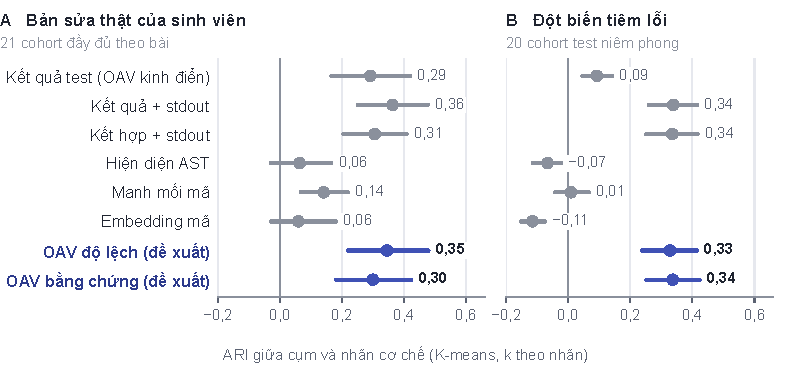
\includegraphics[width=\textwidth]{figures/fig5_ari_vi.pdf}
\caption{RQ2. Chỉ số Rand hiệu chỉnh giữa cụm K-means ($k$ theo nhãn) và nhãn cơ chế. Chàm: biểu diễn đề xuất; xám: baseline. Điểm là trung bình trên các cohort; thanh là khoảng bootstrap 95\% trên các cohort. Bản sửa thật được đánh giá trên cohort đầy đủ theo bài tập (sửa đổi A3), mutant tiêm lỗi trên cohort kiểm tra niêm phong.}\label{fig:ari}
\end{figure}

\begin{table}[t]
\centering
\caption{Khôi phục cơ chế trên hai benchmark: ARI trung bình trên các cohort ($k$ theo nhãn nếu không ghi khác) và trần khả phân biệt trung bình. Bản sửa thật: cohort đầy đủ theo bài tập (sửa đổi A3); mutant tiêm lỗi: cohort của partition kiểm tra niêm phong.}\label{tab:ari}
\small
\begin{tabular}{lrrrr}
\toprule
Biểu diễn & K-means & HAC & K-means, $k$ silhouette & Trần \\
\midrule
\multicolumn{5}{l}{\emph{Bản sửa thật}} \\
{{table_ari_real}}
\midrule
\multicolumn{5}{l}{\emph{Mutant tiêm lỗi}} \\
{{table_ari_injected}}
\bottomrule
\end{tabular}
\end{table}

\paragraph{Cơ chế nào được lợi (khám phá)}
ARI cấp cohort coi trọng nhất các loại lớn, nên chúng tôi đo thêm, theo từng loại, tỷ lệ item có cụm K-means mang đúng loại đó làm nhãn đa số (\cref{fig:categories}). Trên bản sửa thật, chữ ký test nhận ra tốt văn bản in ({{real_rec_outcomes_output_text}}), biên vòng lặp ({{real_rec_outcomes_loop_boundary}}) và luồng điều khiển ({{real_rec_outcomes_control_flow}}), nhưng không nhận ra định dạng in ({{real_rec_outcomes_output_format}}), điều kiện rẽ nhánh ({{real_rec_outcomes_branch_condition}}) hay thiếu bước ({{real_rec_outcomes_missing_statement}}); với OAV độ lệch các giá trị này tăng lên {{real_rec_deviation_output_format}}, {{real_rec_deviation_branch_condition}} và {{real_rec_deviation_missing_statement}}. Tính trung bình theo loại, mức khôi phục tăng từ {{real_catrec_outcomes}} lên {{real_catrec_deviation}} trên bài thật và từ {{injected_catrec_outcomes}} lên {{injected_catrec_deviation}} trên bài tiêm lỗi. Lợi ích của bằng chứng output tập trung ở các cơ chế thiểu số, điều giải thích vì sao chênh lệch ARI trên benchmark thật nhỏ. Phân tích này được thêm sau lần chạy niêm phong (sửa đổi A7) và không phải giả thuyết đã đăng ký.

\begin{figure}[!tbp]
\centering
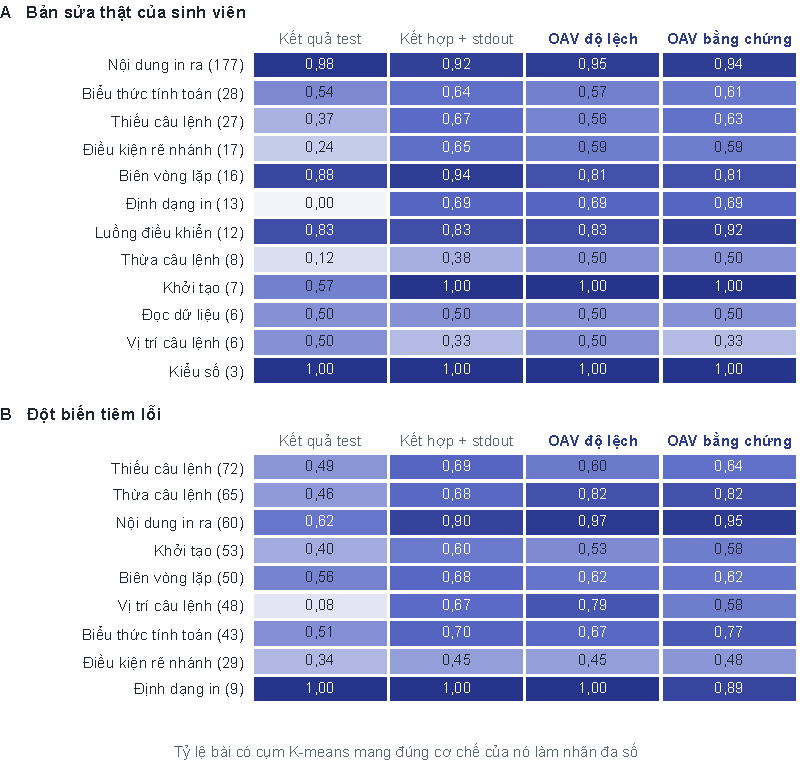
\includegraphics[width=\textwidth]{figures/fig6_categories_vi.pdf}
\caption{RQ2, khám phá. Tỷ lệ item của mỗi cơ chế có cụm K-means ($k$ theo nhãn, seed 42) mang đúng cơ chế đó làm nhãn đa số; số item trong ngoặc. Ô càng đậm, khôi phục càng tốt.}\label{fig:categories}
\end{figure}

\subsection{RQ3: luật NẾU--THÌ}
Luật ILA-2 trên các thuộc tính bằng chứng không phụ thuộc bài dự đoán cơ chế của item thật thuộc partition kiểm tra với macro-F1 {{real_seen_problems_evidence_ila2_macro_f1}} (độ phủ {{real_seen_problems_evidence_ila2_coverage}}, độ chính xác trên item có trả lời {{real_seen_problems_evidence_ila2_selective_accuracy}}), so với {{real_seen_problems_outcome_summary_ila2_macro_f1}} của luật trên tóm tắt kết quả và {{real_seen_problems_majority_macro_f1}} của lớp đa số (\cref{fig:rules,tab:rules}). Chênh lệch {{h4_mean}} [{{h4_lo}}; {{h4_hi}}] chỉ dựa trên {{real_seen_problems_evidence_ila2_n}} item đơn cơ chế của sinh viên kiểm tra và chứa 0, nên H4 không được ủng hộ.

Trên benchmark tiêm lỗi, nơi mọi loại đều có mặt, luật bằng chứng đạt macro-F1 {{injected_seen_problems_evidence_ila2_macro_f1}} trên bài đã thấy và {{injected_unseen_problems_evidence_ila2_macro_f1}} trên bài mới, trong khi luật tóm tắt kết quả đạt {{injected_seen_problems_outcome_summary_ila2_macro_f1}} và {{injected_unseen_problems_outcome_summary_ila2_macro_f1}}: luật chỉ dựa trên trạng thái kết quả hầu như không chuyển được, còn luật dựa trên độ lệch output thì chuyển được. Tập thuộc tính quan trọng hơn thuật toán học. Cây CART trên cùng thuộc tính bằng chứng đạt {{injected_seen_problems_evidence_cart_macro_f1}} và {{injected_unseen_problems_evidence_cart_macro_f1}}, thấp hơn ILA-2 trên bài đã thấy và nhỉnh hơn một chút trên bài mới. Hệ số phạt chịu nhiễu của ILA-2 đổi một chút độ chính xác lấy nhiều độ phủ: ILA gốc trả lời {{injected_seen_problems_evidence_ila_coverage}} item kiểm tra tiêm lỗi với độ chính xác {{injected_seen_problems_evidence_ila_selective_accuracy}}, còn ILA-2 trả lời {{injected_seen_problems_evidence_ila2_coverage}} với độ chính xác {{injected_seen_problems_evidence_ila2_selective_accuracy}}. \Cref{tab:toprules} liệt kê các luật có độ chính xác cao nhất học từ bản sửa thật; chúng đọc giống luật sản xuất của cách phát biểu kinh điển, nhưng kết luận là cơ chế mức chương trình và độ chính xác được đo trên những sinh viên không tham gia quy nạp.

\begin{figure}[tbp]
\centering
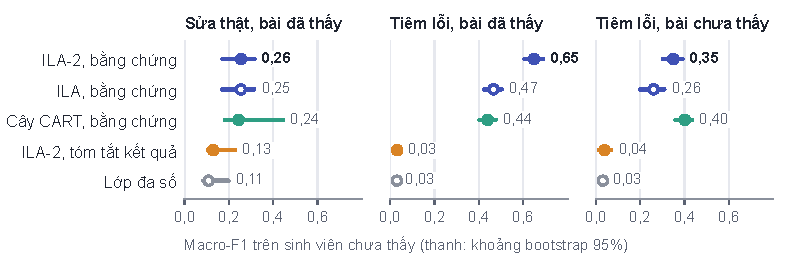
\includegraphics[width=\textwidth]{figures/fig7_rules_vi.pdf}
\caption{RQ3. Macro-F1 của các bộ học luật trên sinh viên chưa thấy, từ chối trả lời được tính là lỗi; thanh là khoảng bootstrap 95\% theo sinh viên. \emph{Bằng chứng}: mô tả độ lệch gộp và manh mối mã; \emph{tóm tắt kết quả}: trạng thái kết quả gộp và tỷ lệ test sai. Bài chưa thấy là các bài của buổi thực hành~4, không có trong dữ liệu huấn luyện.}\label{fig:rules}
\end{figure}

\begin{table}[t]
\centering
\caption{Luật NẾU--THÌ dự đoán cơ chế của sinh viên thuộc partition kiểm tra từ các thuộc tính không phụ thuộc bài, trên bản sửa thật. Từ chối trả lời được tính là lỗi trong macro-F1; độ chính xác chọn lọc đo trên các item có trả lời.}\label{tab:rules}
\small
\resizebox{\textwidth}{!}{%
\begin{tabular}{llrrr}
\toprule
Hướng đánh giá & Mô hình (thuộc tính) & Macro-F1 & Độ phủ & Độ chính xác chọn lọc \\
\midrule
{{table_rules_real}}
\bottomrule
\end{tabular}}
\end{table}

\begin{table}[t]
\centering
\caption{Các luật ILA-2 chính xác nhất quy nạp từ bản sửa thật thuộc partition huấn luyện (hỗ trợ: số item huấn luyện đúng/khớp).}\label{tab:toprules}
\small
\begin{tabular}{p{7.6cm}p{3.0cm}r}
\toprule
NẾU & THÌ cơ chế & Hỗ trợ \\
\midrule
{{table_top_rules}}
\bottomrule
\end{tabular}
\end{table}

\subsection{RQ4: embedding mã đóng băng gom chương trình, không gom cơ chế}
Cụm Qwen3-Embedding của các mutant khớp với chương trình gốc sinh ra mutant nhiều hơn là với cơ chế được tiêm, chênh {{injected_H5_mean}} ARI (KTC 95\% [{{injected_H5_lo}}; {{injected_H5_hi}}]; H5 được ủng hộ). ARI theo cơ chế của chúng là {{injected_ari_embedding}} trên bài tiêm lỗi và {{real_ari_embedding}} trên bài thật (\cref{fig:ari}). Những thay đổi một token quyết định hành vi chương trình hầu như không dịch chuyển một embedding đa dụng, trong khi dấu ấn tác giả và phong cách lời giải chi phối nó.
